\section*{Appendix}

\subsection*{Site split formulation}
We begin by introducing ``site splits.''
One application of site splits is to formalize the notion that a given site pattern is equally probable to its complement under the binary symmetric model.
This is a standard step in the description of the Hadamard transform (Section 8.6 of \citet{Semple2003-em}), although our approach is complicated slightly by the inclusion of ancestral states.

Since we have a finite character alphabet, for a given column $i$ there are a finite number of possible assignments of characters to tips $\alignmentColumn_i$ or internal nodes $\ancestralStateColumn_i$.
For the binary symmetric model, the alphabet $\alphabet$ is $\{0,1\}$.
Take the tip labels of $\tau$ to be $\{1,\ldots,\nSiteRows\}$.
For likelihood calculation under the binary symmetric model, we describe a given $\alignmentColumn_i$ as a subset of indices $\siteSplit\subseteq\siteSplitSet:=\{1,\ldots,\nSiteRows-1\}$, commonly called a ``site split.''
Define the complement of $\alignmentColumn$ as $\overline{\alignmentColumn}$, and let $\alignmentColumn_{i,k}$ be the label of the $k$th tip in the $i$th alignment column.
We define the site split $\siteSplit$ for a $\alignmentColumn_i$ as the set of tips labeled with $1$ in $\alignmentColumn_i$ if the $\nSiteRows$th tip is not labeled with $1$, and as the set of tips labeled with $1$ in $\overline{\alignmentColumn}_i$ if the $\nSiteRows$th tip is labeled with $1$.
Taking such a complement simplifies but does not change the result of likelihood computation because the probability of observing a particular collection of binary characters is equivalent to the probability of its complement under the binary symmetric model.

For a fixed topology $\tau$, we define an ordered set of internal node labels $\{1,\ldots,\nAncestralStateRows\}$ for $\ancestralStateColumn_i$ and similarly use a subset of characters $\ancestralSplit\subseteq\ancestralSplitSet:=\{1,\ldots,\nAncestralStateRows\}$ to describe a realization $\ancestralStateColumn_i$.
In this case we cannot use the same complement trick as before: the probability of observing an ancestral state split conditional on a site split is not invariant to taking its complement.
We thus define an ``ancestral state split'' $\ancestralSplit$ for an internal node $\ancestralStateColumn_i$ to be the set of internal nodes labeled with $1$ if the $\nSiteRows$th tip is not labeled with $1$, and as the set of internal nodes labeled with $1$ in $\overline{\ancestralStateColumn}_i$ if the $\nSiteRows$th tip is labeled with $1$.
We emphasize that the ancestral state split complementing procedure depends on tip states, not ancestral states: both site splits and ancestral state splits are defined by whether the $\nSiteRows$th element of $\alignmentColumn_i$ is labeled as $1$.

We enumerate the site splits $\siteSplit_j$ of which there are $\nSiteSplits=|\mathcal{P}(\siteSplitSet)|$ in total where $\mathcal{P}$ denotes the power set.
Similarly we enumerate ancestral state splits $\ancestralSplit_k$ of which there are $\nAncestralSplits=|\mathcal{P}(\ancestralSplitSet)|$ in total.

We first fix notation.
\begin{definition}
Let the mapping from site patterns to site splits
\[
\patternToSplit:\alphabet^\nSiteRows\rightarrow\mathcal{P}(\siteSplitSet)
\]
be
\[
\patternToSplit(\alignmentColumn) =
\left\{
    \begin{array}{ll}
        \{i'\in\{1,\ldots,\nSiteRows-1\}: \alignmentColumn_{i,i'}=1\}  & \mbox{if } \alignmentColumn_{i,\nSiteRows}\neq 1,\\
        \{i'\in\{1,\ldots,\nSiteRows-1\}: \overline{\alignmentColumn}_{i,i'}=1\}  & \mbox{if } \alignmentColumn_{i,\nSiteRows}=1,
    \end{array}
\right.
\]
and the mapping from ancestral states and tip states to ancestral state splits
\[
\ancestralToSplit:\alphabet^\nSiteRows\times\alphabet^\nAncestralStateRows\rightarrow\mathcal{P}(\ancestralSplitSet)
\]
be
\[
\ancestralToSplit(\alignmentColumn, \ancestralStateColumn) =
\left\{
    \begin{array}{ll}
        \{i'\in\{1,\ldots,\nAncestralStateRows\}: \ancestralStateColumn_{i,i'}=1\}  & \mbox{if } \alignmentColumn_{i,\nSiteRows}\neq 1,\\
        \{i'\in\{1,\ldots,\nAncestralStateRows\}: \overline{\ancestralStateColumn}_{i,i'}=1\}  & \mbox{if } \alignmentColumn_{i,\nSiteRows}=1.
    \end{array}
\right.
\]
Then, given a site pattern--valued random variable $\alignmentColumnRV$ and an ancestral state--valued random variable $\ancestralStateColumnRV$, define the random variables
\[
\siteSplitRV := \patternToSplit(\alignmentColumnRV)
\]
and
\[
\ancestralSplitRV := \ancestralToSplit(\alignmentColumnRV, \ancestralStateColumnRV).
\]
\end{definition}
The mapping $\patternToSplit$ operates by returning the tips labeled as $1$ in a site pattern to obtain a site split in $\mathcal{P}(\siteSplitSet)$ if the set of tips labeled $1$ is not in $\mathcal{P}(\siteSplitSet)$.
The mapping $\ancestralToSplit$ is defined by whether the tip states have their complements taken or not: if the set of tips labeled $1$ in $\alignmentColumn$ is in $\mathcal{P}(\siteSplitSet)$, $\ancestralToSplit(\alignmentColumn, \ancestralStateColumn)$ is the set of tips labeled $1$ in $\ancestralStateColumn$; otherwise, the set of tips labeled $1$ in $\overline{\alignmentColumn}$ necessarily is in $\mathcal{P}(\siteSplitSet)$.

For the $i$th factor of \eqref{eq:full_likelihood},
\[
\Pr(\alignmentColumnRV=\alignmentColumn_i, \ancestralStateColumnRV=\ancestralStateColumn_i \mid \tau, t) = \Pr(\alignmentColumnRV=\alignmentColumn_i \mid \tau, t) \cdot \Pr(\ancestralStateColumnRV=\ancestralStateColumn_i \mid \alignmentColumnRV=\alignmentColumn_i, \tau, t).
\]
As a consequence of assuming a binary symmetric model, for some $\siteSplit_j\in\mathcal{P}(\siteSplitSet)$ the mapping $\patternToSplit(\alignmentColumn_i)$ has the property
\begin{align*}
    \Pr(\siteSplitRV=\siteSplit_j \mid \tau, t) &= \Pr(\siteSplitRV=\patternToSplit(\alignmentColumn_i) \mid \tau, t)\\
    &= \Pr(\alignmentColumnRV=\alignmentColumn_i \cup \overline{\alignmentColumnRV}=\alignmentColumn_i \mid \tau, t)\\
    &= \Pr(\alignmentColumnRV=\alignmentColumn_i \mid \tau, t) + \Pr(\overline{\alignmentColumnRV}=\alignmentColumn_i \mid \tau, t)\\
    &= 2\cdot\Pr(\alignmentColumnRV=\alignmentColumn_i \mid \tau, t)
\end{align*}
where $\overline{Y}$ is the complement of the site pattern--valued random variable $Y$ and has the same distribution as $Y$.
Note
\begin{align*}
    \Pr(\ancestralStateColumnRV=\ancestralStateColumn_i \mid \alignmentColumnRV=\alignmentColumn_i, \tau, t) &= \Pr(\ancestralSplitRV=\ancestralToSplit(\alignmentColumn_i, \ancestralStateColumn_i) \mid \siteSplitRV=\patternToSplit(\alignmentColumn_i), \tau, t).
\end{align*}
Thus given $(\tau, t)$, there exist sets $\ancestralSplitPartition_1(\tau, t),\ldots,\ancestralSplitPartition_\nSiteSplits(\tau, t)$ such that $\xi_j\in\ancestralSplitPartition_j(\tau, t)$ satisfies
\begin{align*}
\max_{\ancestralSplit_k\in\mathcal{P}(\ancestralSplitSet)} \ \Pr(\ancestralSplitRV=\ancestralSplit_k \mid \siteSplitRV=\siteSplit_j, \tau, t) &= \Pr(\ancestralSplitRV = \xi_j \mid \siteSplitRV=\siteSplit_j, \tau, t).
\end{align*}
In other words, for the $j$th site split, $\ancestralSplitPartition_j(\tau, t)\subseteq\mathcal{P}(\ancestralSplitSet)$ is the set of most likely ancestral state splits for that particular site split, topology and set of branch lengths, i.e., $\ancestralSplitPartition_j(\tau, t)$ is a set of sets of most likely internal node labels.
Here, $\xi_j$ is one of possibly many equiprobable ancestral state splits in $\ancestralSplitPartition_j(\tau, t)$.
For each $\alignmentColumn_i$, $\ancestralToSplit(\alignmentColumn_i, \cdot)$ is surjective as it can map values from $\alphabet^\nAncestralStateRows$ to all elements in $\mathcal{P}(\ancestralSplitSet)$.
This can be seen by using the definition of $\ancestralToSplit(\alignmentColumn_i, \cdot)$ and assuming $\alignmentColumn_{i,\nSiteRows}\neq 1$, where in this case each of the $2^\nAncestralStateRows$ values of $\ancestralStateColumn$ correspond to each of the $2^\nAncestralStateRows$ elements of $\mathcal{P}(\{1,\ldots,\nAncestralStateRows\})$.
The same can be done for the case of $\alignmentColumn_{i,\nSiteRows}=1$, implying $\ancestralToSplit(\alignmentColumn_i, \cdot)$ is surjective.
From this we have
\begin{align*}
    \max_{\ancestralStateColumn_i} \ \Pr(\ancestralStateColumnRV=\ancestralStateColumn_i \mid \alignmentColumnRV=\alignmentColumn_i, \tau, t) &= \max_{\ancestralStateColumn_i} \ \Pr(\ancestralSplitRV=\ancestralToSplit(\alignmentColumn_i, \ancestralStateColumn_i) \mid \siteSplitRV=\patternToSplit(\alignmentColumn_i), \tau, t)\\
    &= \max_{\ancestralSplit_k\in\mathcal{P}(\ancestralSplitSet)} \ \Pr(\ancestralSplitRV=\ancestralSplit_k \mid \siteSplitRV=\siteSplit_j, \tau, t)\\
    &= \Pr(\ancestralSplitRV = \xi_j \mid \siteSplitRV=\siteSplit_j, \tau, t)
\end{align*}
for some $j$.
Thus, each term in the likelihood can be collapsed into terms relating only to site splits and ancestral state splits, indexed by $j$, as opposed to individual observations, indexed by $i$.

\subsection*{Example}
We follow with an expository example computing these probabilities and likelihoods.
Consider the fixed, binary four-taxon tree $\tau_1$ in Fig.~\ref{fig:farris-fels-top}a.
The set of all possible character assignments is
\begin{align*}
\mathcal{P}(\{1,2,3,4\}) &= \{\emptyset, \{1,2,3,4\}, \{1\}, \{2,3,4\}, \{2\}, \{1,3,4\}, \{3\}, \{1,2,4\}, \\
                         &\qquad \{1,2\}, \{3,4\}, \{1,3\}, \{2,4\}, \{2,3\}, \{1,4\}, \{1,2,3\}, \{1,4\}\}
\end{align*}
where each set indicates the tips assigned the character $1$.
For example, $\emptyset$ is the labeling $0000$ and $\{1,3,4\}$ is the labeling $1011$.
Symmetry allows us to group adjacent pairs in $\mathcal{P}(\{1,2,3,4\})$ into equiprobable splits, letting $\siteSplitSet=\{1,2,3\}$.
The unique site splits, collapsing complements, are
\begin{align*}
    \mathcal{P}(\siteSplitSet) &= \{\emptyset, \{1\}, \{2\}, \{3\}, \{1,2\}, \{1,3\}, \{2,3\}, \{1,2,3\}\} \\
& := \{\siteSplit_1, \ldots, \siteSplit_8\}.
\end{align*}
Since we identify character complements, we do not consider the additional splits
\begin{equation*}
\begin{split}
& \mathcal{P}(\{1,2,3,4\}) \setminus \mathcal{P}(\siteSplitSet) = \\
&\qquad \{\{1,2,3,4\}, \{2,3,4\}, \{1,3,4\}, \{1,2,4\}, \{3,4\}, \{2,4\}, \{1,4\}, \{4\}\},
\end{split}
\end{equation*}
the symmetry of the binary character model allowing us to focus only on the elements of $\mathcal{P}(\siteSplitSet)$.
This tree has two internal nodes with $\ancestralSplitSet=\{1,2\}$ and unique ancestral state splits
\[
\mathcal{P}(\ancestralSplitSet) = \{\emptyset, \{1\}, \{2\}, \{1,2\}\}.
\]
Internal node $1$ is the node connected to leaves $1$ and $3$ while internal node $2$ is connected to leaves $2$ and $4$.
The mapping from characters to splits in this case will depend on the characters at the tips and the ancestral states.
For example, we take both $\patternToSplit(0000)=\emptyset$ and $\patternToSplit(1111)=\emptyset$.
Similarly, we have $\ancestralToSplit(0000, 00) = \emptyset$ and $\ancestralToSplit(1111, 11)=\emptyset$, needing to take the complement of all the characters present on the tree to identify splits.
We cannot identify complements for ancestral states in the same way as tip states since, for $\siteSplit\in\mathcal{P}(\siteSplitSet)$,
\[
\Pr(\ancestralSplitRV=\emptyset \mid \siteSplitRV=\siteSplit, \tau, t)\neq \Pr(\ancestralSplitRV=\{1,2\} \mid \siteSplitRV=\siteSplit, \tau, t)
\]
in general.

For each site split $\siteSplit\in\mathcal{P}(\siteSplitSet)$, we maximize the likelihood over all $\ancestralSplit\in\mathcal{P}(\ancestralSplitSet)$.
A maximum occurs at one of possibly several ancestral state splits in $\mathcal{P}(\ancestralSplitSet)$, defined via $\ancestralSplitPartition_j(\tau, t)$ for the $j$th site split.
As a simple example, say all branch lengths correspond to a probability $p$ ($< 1/2$) of changing character along that branch, with $t=\{p,p,p,p,p\}$.
The probabilities of observing ancestral state splits for $\siteSplit_1=\emptyset$ are
\[
\Pr(\ancestralSplitRV=\emptyset \mid \siteSplitRV=\emptyset, \tau, t) =
(1-p)^5,
\]
\[
\Pr(\ancestralSplitRV=\{1\} \mid \siteSplitRV=\emptyset, \tau, t) =
\Pr(\ancestralSplitRV=\{2\} \mid \siteSplitRV=\emptyset, \tau, t) =
p^3(1-p)^2,
\]
\[
\Pr(\ancestralSplitRV=\{1,2\} \mid \siteSplitRV=\emptyset, \tau, t) =
p^4(1-p).
\]
The set of most likely ancestral states contains a single element, here $\ancestralSplitPartition_1(\tau, t)=\{\emptyset\}$.
Then, taking $\xi_1\in\ancestralSplitPartition_1(\tau, t)$ we have
\[
\Pr(\ancestralSplitRV=\xi_1 \mid \siteSplitRV=\emptyset, \tau, t) =
\Pr(\ancestralSplitRV=\emptyset \mid \siteSplitRV=\emptyset, \tau, t) =
(1-p)^5.
\]
For $\siteSplit_5=\{1,2\}$ we have
\[
\Pr(\ancestralSplitRV=\emptyset \mid \siteSplitRV=\{1,2\}, \tau, t) =
\Pr(\ancestralSplitRV=\{1,2\} \mid \siteSplitRV=\{1,2\}, \tau, t) =
p^2(1-p)^3,
\]
\[
\Pr(\ancestralSplitRV=\{1\} \mid \siteSplitRV=\{1,2\}, \tau, t) =
\Pr(\ancestralSplitRV=\{2\} \mid \siteSplitRV=\{1,2\}, \tau, t) =
p^3(1-p)^2.
\]
Here, the set of most likely ancestral states is $\ancestralSplitPartition_5(\tau, t)=\{\emptyset,\{1,2\}\}$, and, for $\xi_5\in\ancestralSplitPartition_5(\tau, t)$,
\[
\Pr(\ancestralSplitRV=\xi_5 \mid \siteSplitRV=\{1,2\}, \tau, t) =
p^2(1-p)^3.
\]

\subsection*{Site split likelihood}

The likelihood in \eqref{eq:profile_likelihood} can be written as
\begin{align}
L_\nCols'(\tau, t; \fullAlignment) &= \max_{\fullAncestralStates} \ L_\nCols(\tau, t; \fullAlignment, \fullAncestralStates) \nonumber \\
                             &= \prod_{i=1}^{\nCols} \ \max_{\ancestralStateColumn_i} \ \Pr(\alignmentColumnRV=\alignmentColumn_i, \ancestralStateColumnRV=\ancestralStateColumn_i \mid \tau, t) \nonumber \\
                             &\propto \prod_{i=1}^{\nCols} \ \max_{\ancestralStateColumn_i} \ \Pr(\siteSplitRV=\patternToSplit(\alignmentColumn_i) \mid \tau, t) \cdot \Pr(\ancestralSplitRV=\ancestralToSplit(\alignmentColumn_i, \ancestralStateColumn_i) \mid \siteSplitRV=\patternToSplit(\alignmentColumn_i), \tau, t) \nonumber \\
                             &= \prod_{i=1}^{\nCols} \ \Pr(\siteSplitRV=\patternToSplit(\alignmentColumn_i) \mid \tau, t) \cdot \max_{\ancestralStateColumn_i} \Pr(\ancestralSplitRV=\ancestralToSplit(\alignmentColumn_i, \ancestralStateColumn_i) \mid \siteSplitRV=\patternToSplit(\alignmentColumn_i), \tau, t) \nonumber \\
                             &= \prod_{j=1}^{\nSiteSplits} \ \left[\Pr(\siteSplitRV=\siteSplit_j \mid \tau, t)\cdot \Pr(\ancestralSplitRV=\xi_j \mid \siteSplitRV=\siteSplit_j, \tau, t)\right] ^{\nCols_j(\fullAlignment)} \label{eq:site_pattern_likelihood}
\end{align}
for $\siteSplit_j\in\mathcal{P}(\siteSplitSet)$ and some $\xi_j\in\ancestralSplitPartition_j(\tau, t)$ with $1 \le j \le q$ where $\nCols_j(\fullAlignment)$ is the number of columns in $\fullAlignment$ that project to site split $\siteSplit_j$.

Let
\[
L_\nCols''(\tau, t; \fullAlignment) = \prod_{j=1}^{\nSiteSplits} \ \left[\Pr(\siteSplitRV=\siteSplit_j \mid \tau, t) \cdot \Pr(\ancestralSplitRV=\xi_j \mid \siteSplitRV=\siteSplit_j, \tau, t)\right] ^{\nCols_j(\fullAlignment)}
\]
be the final product in \eqref{eq:site_pattern_likelihood}.
Assume $\nCols$ observations are generated from a model with parameters $(\tau^*, t^*)$.
We have
\begin{equation*}
\begin{split}
&    \frac{1}{\nCols} \log L_\nCols''(\tau, t; \fullAlignment) \\
&\qquad = \sum_{j=1}^\nSiteSplits \frac{\nCols_j(\fullAlignment)}{\nCols}\cdot  \log \Pr(\siteSplitRV=\siteSplit_j, \ancestralSplitRV=\xi_j \mid \tau, t) \\
&\qquad = \sum_{j=1}^\nSiteSplits \frac{\nCols_j(\fullAlignment)}{\nCols}\cdot [\log \Pr(\siteSplitRV=\siteSplit_j \mid \tau, t) +
            \log \Pr(\ancestralSplitRV=\xi_j \mid \siteSplitRV=\siteSplit_j , \tau, t)]
\end{split}
\end{equation*}
so that, in the $\nCols\rightarrow\infty$ limit,
\begin{equation}
\begin{split}
&    \frac{1}{\nCols} \log L_\nCols''(\tau, t; \fullAlignment) \\
&\qquad \rightarrow \sum_{j=1}^\nSiteSplits \Pr(\siteSplitRV=\siteSplit_j \mid \tau^*, t^*) \cdot [\log \Pr(\siteSplitRV=\siteSplit_j \mid \tau, t) + \log \Pr(\ancestralSplitRV=\xi_j \mid \siteSplitRV=\siteSplit_j , \tau, t)]. \label{eq:site_pattern_profile_likelihood_mean}
\end{split}
\end{equation}
Define the divergence quantity
\[
\shannonDivergence_{\tau^*,t^*}(\tau,t) = \sum_{j=1}^\nSiteSplits \Pr(\siteSplitRV=\siteSplit_j \mid \tau^*, t^*)\cdot\log \Pr(\siteSplitRV=\siteSplit_j \mid \tau, t)
\]
and the partial log-likelihood
\[
\tilde{\ell}_{\tau^*,t^*}(\tau, t) = \sum_{j=1}^\nSiteSplits \Pr(\siteSplitRV=\siteSplit_j \mid \tau^*, t^*)\cdot\log \Pr(\ancestralSplitRV=\xi_j \mid \siteSplitRV = \siteSplit_j, \tau, t)
\]
so that \eqref{eq:site_pattern_profile_likelihood_mean} is
\begin{equation}
    \label{eq:log_likelihood_simplified}
    \ell_{\tau^*,t^*}(\tau, t) = \shannonDivergence_{\tau^*,t^*}(\tau,t) + \tilde{\ell}_{\tau^*,t^*}(\tau, t).
\end{equation}

\subsection*{Hadamard representation}

We state the Hadamard representation of site split generating probabilities---that is, probabilities of obtaining particular site splits given a tree---following Section 8.6 of \citet{Semple2003-em}.
For each edge $e$ define the edge ``fidelity'' for that edge as
\[
\theta(e) = 1-2p(e)
\]
where $p(e)$ is the probability of a character change along edge $e$.
For an even-sized subset of $Y\subseteq\mathcal{S}$, let the path set $P(Y)$ be the set of edges in the path connecting both elements of $Y$.
For $n$ taxa, the probability of observing site split $A\in\mathcal{P}(\siteSplitSet)$ is
\begin{equation}
\label{eq:hadamard_probability}
p_A = \frac{1}{2^{n-1}} \ \sum_{Y \subseteq \mathcal{S} : |Y| \equiv 0 (\mathrm{mod} \ 2)} \ \left[(-1)^{|Y \cap A|} \ \prod_{e\in P(Y)} \ \theta(e) \right].
\end{equation}
By convention, we set $P(\emptyset)=\emptyset$ and $\prod_{e\in\emptyset} \ \theta(e) = 1$.
For notational convenience, let
\[
p_{\siteSplit_j} := \Pr(\siteSplitRV=\siteSplit_j \mid \tau_1,t),
\]
for any site split $\siteSplit_j$.
Table~\ref{tab:gen-sitepatprob} contains calculations of site split probabilities for the InvFels topology with arbitrary branch lengths and Table~\ref{tab:sitepatprob} site split probabilities for the InvFels topology in Fig.~\ref{fig:farris-fels-top}a.

\begin{table}[ht]
\centering
\begin{tabular}{|l|l|l|}
    \hline
$\siteSplit_j$  & $p_{\siteSplit_j}$ &$\Pr(\siteSplitRV=\siteSplit_j \mid \tau_1,\{x_1,y_1,x_2,y_2,w\})$\\
    \hline
    $\emptyset$ & $p_{\emptyset}$   &$1 + x_1x_2 +  y_1y_2 +  w[  x_1 + x_2][  y_1 + y_2] + x_1y_1x_2y_2$\\
    $\{1\}$     & $p_{1}$       &$1 - x_1x_2 +  y_1y_2 +  w[- x_1 + x_2][  y_1 + y_2] - x_1y_1x_2y_2$\\
    $\{2\}$     & $p_{2}$       &$1 + x_1x_2 -  y_1y_2 +  w[  x_1 + x_2][- y_1 + y_2] - x_1y_1x_2y_2$\\
    $\{3\}$     & $p_{3}$       &$1 - x_1x_2 +  y_1y_2 +  w[  x_1 - x_2][  y_1 + y_2] - x_1y_1x_2y_2$\\
    $\{1,2\}$   & $p_{12}$     &$1 - x_1x_2 -  y_1y_2 +  w[- x_1 + x_2][- y_1 + y_2] + x_1y_1x_2y_2$\\
    $\{1,3\}$   & $p_{13}$     &$1 + x_1x_2 +  y_1y_2 +  w[- x_1 - x_2][  y_1 + y_2] + x_1y_1x_2y_2$\\
    $\{2,3\}$   & $p_{23}$     &$1 - x_1x_2 -  y_1y_2 +  w[  x_1 - x_2][- y_1 + y_2] + x_1y_1x_2y_2$\\
    $\{1,2,3\}$ & $p_{123}$   &$1 + x_1x_2 -  y_1y_2 +  w[  x_1 + x_2][  y_1 - y_2] - x_1y_1x_2y_2$\\
    \hline
\end{tabular}
\caption{Site split probabilities $p_{\siteSplit_j}$ on the InvFels tree $\tau_1$ with $t=\{x_1,y_1,x_2,y_2,w\}$ obtained using the Hadamard transform.
All values multiplied by $1/8$.}
\label{tab:gen-sitepatprob}
\end{table}

\begin{table}[ht]
\centering
\begin{tabular}{|l|l|l|}
    \hline
$\siteSplit_j$  & $p_{\siteSplit_j}$ &$\Pr(\siteSplitRV=\siteSplit_j \mid \tau_1,\{x,y,x,y,y\})$\\
    \hline
    $\emptyset$ & $p_{\emptyset}$   &$1+x^2+y^2+4xy^2+x^2y^2$\\
    $\{1\}$     & $p_{1}$           &$1-x^2+y^2-x^2y^2$\\
    $\{2\}$     & $p_{2}$           &$1+x^2-y^2-x^2y^2$\\
    $\{3\}$     & $p_{3}$           &$1-x^2+y^2-x^2y^2$\\
    $\{1,2,3\}$ & $p_{123}$         &$1+x^2-y^2-x^2y^2$\\
    $\{1,2\}$   & $p_{12}$          &$1-x^2-y^2+x^2y^2$\\
    $\{2,3\}$   & $p_{23}$          &$1-x^2-y^2+x^2y^2$\\
    $\{1,3\}$   & $p_{13}$          &$1+x^2+y^2-4xy^2+x^2y^2$\\
    \hline
\end{tabular}
\caption{Site split probabilities $p_{\siteSplit_j}$ on the InvFels tree $\tau_1$ with $t=\{x,y,x,y,y\}$ obtained using the Hadamard transform.
All values multiplied by $1/8$.}
\label{tab:sitepatprob}
\end{table}

\subsection*{Likelihood computations}

To compute the likelihood of observing a set of data, we need $\Pr(\ancestralSplitRV=\ancestralSplit_k \mid \siteSplitRV=\siteSplit_j, \tau, t)$ for each $\ancestralSplit_k$ and $\siteSplit_j$.
Using branch fidelities, the probability of a character change along a branch with fidelity parameter $\theta$ is $(1-\theta)/2$, while the probability of a character remaining the same is $(1+\theta)/2$.
See Fig.~\ref{fig:example_likelihoods} for the parameters on an example site pattern on the InvFels tree.
Likelihood computations for all site splits and ancestral state splits are in Table~\ref{tab:farris_likelihoods} for the InvFels tree.
Taking maxima over ancestral state splits results in Table~\ref{tab:likelihoods}.

\begin{figure}
\centering
\begin{subfigure}{.45\linewidth}
\centering
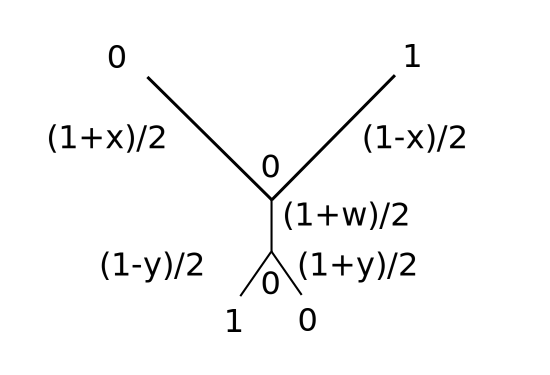
\includegraphics[width=.95\textwidth]{farris_like00}
\caption[short]{}
\end{subfigure}
\begin{subfigure}{.45\linewidth}
\centering
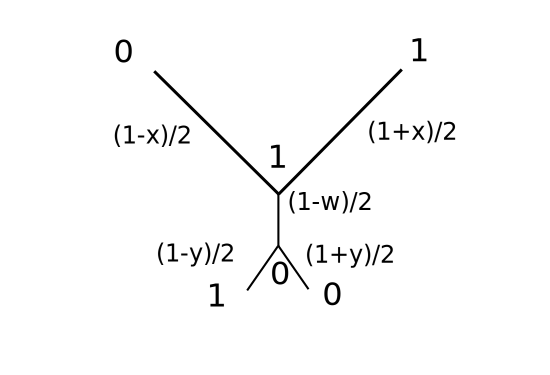
\includegraphics[width=.95\textwidth]{farris_like10}
\caption[short]{}
\end{subfigure}
\caption{
    Example likelihood computations on the InvFels tree $\tau_1$ for fidelities $\{x_1,y_1,x_2,y_2,w\}$.
    Edges labeled by the probability of substitution along that edge.
    In (a), we compute the product to obtain $\Pr(\ancestralSplitRV=\emptyset\mid \siteSplitRV=\{2,3\},\tau_1,t) = (1+x_1)(1-x_2)(1+y_1)(1-y_2)(1+w)/32$.
    In (b), the same process yields $\Pr(\ancestralSplitRV=\{1\}\mid \siteSplitRV=\{2,3\},\tau_1,t) = (1+x_1)(1-x_2)(1+y_1)(1-y_2)(1-w)/32$.
}
\label{fig:example_likelihoods}
\end{figure}

\begin{table}
\centering
\begin{tabular}{|ll|l|}
\hline
$\siteSplit_j$ & $\ancestralSplit_k$ & $\Pr(\ancestralSplitRV=\ancestralSplit_k \mid \siteSplitRV=\siteSplit_j, \tau_1, t)$\\
\hline
$\emptyset$&$\emptyset$&$(1+x_1)(1+y_1)(1+x_2)(1+y_2)(1+w)$\\
&$\{1\}^*$&$(1-x_1)(1+y_1)(1-x_2)(1+y_2)(1-w)$\\
&$\{2\}^*$&$(1+x_1)(1-y_1)(1+x_2)(1-y_2)(1-w)$\\
&$\{1,2\}^*$&$(1-x_1)(1-y_1)(1-x_2)(1-y_2)(1+w)$\\

$\{1\}$    &$\emptyset$&$(1-x_1)(1+y_1)(1+x_2)(1+y_2)(1+w)$\\
&$\{1\}$&$(1+x_1)(1+y_1)(1-x_2)(1+y_2)(1-w)$\\
&$\{2\}^*$&$(1-x_1)(1-y_1)(1+x_2)(1-y_2)(1-w)$\\
&$\{1,2\}$&$(1+x_1)(1-y_1)(1-x_2)(1-y_2)(1+w)$\\

$\{2\}$    &$\emptyset$&$(1+x_1)(1-y_1)(1+x_2)(1+y_2)(1+w)$\\
&$\{1\}^*$&$(1-x_1)(1-y_1)(1-x_2)(1+y_2)(1-w)$\\
&$\{2\}$&$(1+x_1)(1+y_1)(1+x_2)(1-y_2)(1-w)$\\
&$\{1,2\}$&$(1-x_1)(1+y_1)(1-x_2)(1-y_2)(1+w)$\\

$\{3\}$    &$\emptyset$&$(1+x_1)(1+y_1)(1-x_2)(1+y_2)(1+w)$\\
&$\{1\}$&$(1-x_1)(1+y_1)(1+x_2)(1+y_2)(1-w)$\\
&$\{2\}^*$&$(1+x_1)(1-y_1)(1-x_2)(1-y_2)(1-w)$\\
&$\{1,2\}$&$(1-x_1)(1-y_1)(1+x_2)(1-y_2)(1+w)$\\

$\{1,2,3\}$&$\emptyset$&$(1-x_1)(1-y_1)(1-x_2)(1+y_2)(1+w)$\\
&$\{1\}$&$(1+x_1)(1-y_1)(1+x_2)(1+y_2)(1-w)$\\
&$\{2\}^*$&$(1-x_1)(1+y_1)(1-x_2)(1-y_2)(1-w)$\\
&$\{1,2\}$&$(1+x_1)(1+y_1)(1+x_2)(1-y_2)(1+w)$\\

$\{1,2\}$  &$\emptyset$&$(1-x_1)(1-y_1)(1+x_2)(1+y_2)(1+w)$\\
&$\{1\}$&$(1+x_1)(1-y_1)(1-x_2)(1+y_2)(1-w)$\\
&$\{2\}$&$(1-x_1)(1+y_1)(1+x_2)(1-y_2)(1-w)$\\
&$\{1,2\}$&$(1+x_1)(1+y_1)(1-x_2)(1-y_2)(1+w)$\\

$\{1,3\}$  &$\emptyset$&$(1-x_1)(1+y_1)(1-x_2)(1+y_2)(1+w)$\\
&$\{1\}$&$(1+x_1)(1+y_1)(1+x_2)(1+y_2)(1-w)$\\
&$\{2\}^*$&$(1-x_1)(1-y_1)(1-x_2)(1-y_2)(1-w)$\\
&$\{1,2\}$&$(1+x_1)(1-y_1)(1+x_2)(1-y_2)(1+w)$\\

$\{2,3\}$  &$\emptyset$&$(1+x_1)(1-y_1)(1-x_2)(1+y_2)(1+w)$\\
&$\{1\}$&$(1-x_1)(1-y_1)(1+x_2)(1+y_2)(1-w)$\\
&$\{2\}$&$(1+x_1)(1+y_1)(1-x_2)(1-y_2)(1-w)$\\
&$\{1,2\}$&$(1-x_1)(1+y_1)(1+x_2)(1-y_2)(1+w)$\\
\hline
\end{tabular}
\caption{
Likelihood calculations for all site splits $\siteSplit_j$ and ancestral state splits $\ancestralSplit_k$ of the InvFels tree $\tau_1$.
All values multiplied by $1/32$.
Ancestral states with $^*$ are never maximal provided parameters are in $(0,1)$.
There are $3^5\cdot 4^2=3,888$ possible forms for the likelihood.
}
\label{tab:farris_likelihoods}
\end{table}

\begin{table}
\centering
\begin{tabular}{|ll|l|}
\hline
$\siteSplit_j$ & $\ancestralSplitPartition_j(\tau, t)$ & $\Pr(\ancestralSplitRV=\xi_j \mid \siteSplitRV=\siteSplit_j,\tau,t)$\\
\hline
$\emptyset$&$\emptyset$&$(1+x_1)(1+y_1)(1+x_2)(1+y_2)(1+w)$\\

$\{1\}$    &$\emptyset$&$(1-x_1)(1+y_1)(1+x_2)(1+y_2)(1+w)$\\

$\{2\}$    &$\emptyset$&$(1+x_1)(1-y_1)(1+x_2)(1+y_2)(1+w)$\\

$\{3\}$    &$\emptyset$&$(1+x_1)(1+y_1)(1-x_2)(1+y_2)(1+w)$\\
&$\{1\}$&$(1-x_1)(1+y_1)(1+x_2)(1+y_2)(1-w)$\\
&$\{1,2\}$&$(1-x_1)(1-y_1)(1+x_2)(1-y_2)(1+w)$\\

$\{1,2,3\}$&$\emptyset$&$(1-x_1)(1-y_1)(1-x_2)(1+y_2)(1+w)$\\
&$\{1\}$&$(1+x_1)(1-y_1)(1+x_2)(1+y_2)(1-w)$\\
&$\{1,2\}$&$(1+x_1)(1+y_1)(1+x_2)(1-y_2)(1+w)$\\

$\{1,2\}$  &$\emptyset$&$(1-x_1)(1-y_1)(1+x_2)(1+y_2)(1+w)$\\

$\{1,3\}$  &$\emptyset$&$(1-x_1)(1+y_1)(1-x_2)(1+y_2)(1+w)$\\
&$\{1\}$&$(1+x_1)(1+y_1)(1+x_2)(1+y_2)(1-w)$\\
&$\{1,2\}$&$(1+x_1)(1-y_1)(1+x_2)(1-y_2)(1+w)$\\

$\{2,3\}$  &$\emptyset$&$(1+x_1)(1-y_1)(1-x_2)(1+y_2)(1+w)$\\
&$\{1\}$&$(1-x_1)(1-y_1)(1+x_2)(1+y_2)(1-w)$\\
&$\{1,2\}$&$(1-x_1)(1+y_1)(1+x_2)(1-y_2)(1+w)$\\
\hline
\end{tabular}
\caption{
Due to the symmetry of the likelihood, WLOG we assume $x_2 \ge x_1$ and $y_2 \ge y_1$ and maximize over ancestral states to reduce the number of possible functional forms to consider.
All values multiplied by $1/32$.
Likelihoods with multiple entries have maxima determined by unknown branch length parameters.
There are $3^4=81$ possible forms for the likelihood.
}
\label{tab:likelihoods}
\end{table}
%TODO: the caption of this overlaps with the page number---will this be a problem or will MBE handle it?
%EM There is a latex package for that, which I tried out and then removed for some reason. It's no bigs.

\subsection*{Properties of the joint objective function}

Consider the InvFels tree $\tau_1$ with arbitrary fidelities, i.e., $\tilde{t}=\{x_1,y_1,x_2,y_2,w\}$.
We show that the likelihood remains unchanged if $x_1$ and $x_2$ are exchanged or if $y_1$ and $y_2$ are.
Using the Hadamard transform, we calculate the generating probabilities on the InvFels tree.
For site split $\emptyset$,
\begin{align*}
    \Pr(\siteSplitRV=\emptyset\mid \tau_1, \tilde{t}) & = \frac{1}{8} (1 + x_1x_2 +  y_1y_2 +  x_1y_1w + x_1y_2w + y_1x_2w + x_2y_2w + x_1y_1x_2y_2) \\
                                              & = \frac{1}{8} (1 + x_1x_2 +  y_1y_2 +  w[x_1y_1 + x_1y_2 + y_1x_2 + x_2y_2] + x_1y_1x_2y_2) \\
                                              & = \frac{1}{8} (1 + x_1x_2 +  y_1y_2 +  w[x_1 + x_2][y_1 + y_2] + x_1y_1x_2y_2),
\end{align*}
and this probability is unchanged when $x_1$ is exchanged with $x_2$ and $y_1$ is exchanged with $y_2$.
All other generating probabilities differ only in the signs of each term (see Table~\ref{tab:gen-sitepatprob}).
For example, for site split $\{1\}$ we have
\begin{align*}
    \Pr(\siteSplitRV=\{1\}\mid \tau_1, \tilde{t}) & = \frac{1}{8} (1 - x_1x_2 +  y_1y_2 +  w[-x_1 + x_2][y_1 + y_2] - x_1y_1x_2y_2)
\end{align*}
and for site split $\{3\}$ we have
\begin{align*}
    \Pr(\siteSplitRV=\{3\}\mid \tau_1, \tilde{t}) & = \frac{1}{8} (1 - x_1x_2 +  y_1y_2 +  w[x_1 - x_2][y_1 + y_2] - x_1y_1x_2y_2)
\end{align*}
meaning if we exchange the values of $x_1$ and $x_2$ then these probabilities swap values.
The corresponding possibilities for the likelihood values are
\begin{align*}
    \Pr(\ancestralSplitRV=\emptyset \mid \siteSplitRV=\{1\}, \tau_1, \tilde{t}) &= \frac{1}{32}(1-x_1)(1+x_2)(1+w)(1+y_1)(1+y_2); \\
    \Pr(\ancestralSplitRV=\{1\} \mid \siteSplitRV=\{1\}, \tau_1, \tilde{t}) &= \frac{1}{32}(1+x_1)(1-x_2)(1-w)(1+y_1)(1+y_2); \\
    \Pr(\ancestralSplitRV=\{2\} \mid \siteSplitRV=\{1\}, \tau_1, \tilde{t}) &= \frac{1}{32}(1-x_1)(1+x_2)(1-w)(1-y_1)(1-y_2); \\
    \Pr(\ancestralSplitRV=\{1,2\} \mid \siteSplitRV=\{1\}, \tau_1, \tilde{t}) &= \frac{1}{32}(1+x_1)(1-x_2)(1+w)(1-y_1)(1-y_2);
\end{align*}
for site split $\{1\}$ and
\begin{align*}
        \Pr(\ancestralSplitRV=\emptyset \mid \siteSplitRV=\{3\}, \tau_1, \tilde{t}) &= \frac{1}{32}(1+x_1)(1-x_2)(1+w)(1+y_1)(1+y_2); \\
    \Pr(\ancestralSplitRV=\{1\} \mid \siteSplitRV=\{3\}, \tau_1, \tilde{t}) &= \frac{1}{32}(1-x_1)(1+x_2)(1-w)(1+y_1)(1+y_2); \\
    \Pr(\ancestralSplitRV=\{2\} \mid \siteSplitRV=\{3\}, \tau_1, \tilde{t}) &= \frac{1}{32}(1+x_1)(1-x_2)(1-w)(1-y_1)(1-y_2); \\
    \Pr(\ancestralSplitRV=\{1,2\} \mid \siteSplitRV=\{3\}, \tau_1, \tilde{t}) &= \frac{1}{32}(1-x_1)(1+x_2)(1+w)(1-y_1)(1-y_2);
\end{align*}
for site split $\{3\}$, which also both swap values when $x_1$ and $x_2$ are exchanged.

The same can be done for the splits $\{2\}$ and $\{1,2,3\}$ by exchanging $y_1$ and $y_2$ as well as $\{1,2\}$ and $\{1,3\}$ by exchanging both $x_1$ with $x_2$ and $y_1$ with $y_2$.
The split $\{1,3\}$ is unchanged by exchanging $x_1$ with $x_2$ and $y_1$ with $y_2$.
Since exchanging $x_1$ and $x_2$ does not change the value of the log-likelihood $\ell_{\tau_1,t^*}(\tau_1, \tilde{t})$, if there is a unique maximum of the log-likelihood then $x_1=x_2$ at the maximum.
An analogous statement holds for $y_1$ and $y_2$.

\subsection*{Theorems and proofs}

%where data is generated on the InvFels tree with two top branches of fidelity $x^*$ and all other branches of fidelity $y^*$ (Fig.~\ref{fig:farris-fels-top}).

We first prove intermediate results to show the above.

\begin{lemma}
Let $t^*=\{x^*, y^*, x^*, y^*, y^*\}$ and $t=\{x_1, y_1, x_2, y_2, w\}$.
There exists a set of $0 < x^*, y^* < 1$ such that $\emptyset$ is the maximal ancestral state for all site splits.
\end{lemma}

\begin{proof}
We obtain
\[
\max_{t} \ \ell_{\tau^*,t^*}(\tau^*, t) \le
    \shannonDivergence_{\tau^*,t^*}(\tau^*,t^*)
    + \tilde{\ell}_{\tau^*,t^*}(\tau^*, \hat{t})
\]
as an upper bound for the joint maximum of \eqref{eq:log_likelihood_simplified} using Gibbs's inequality
\[
\shannonDivergence_{\tau^*,t^*}(\tau^*,t) \le \shannonDivergence_{\tau^*,t^*}(\tau^*,t^*)
\]
and
\[
\hat{t} = \argmax_{t} \ \tilde{\ell}_{\tau^*,t^*}(\tau^*, t).
\]
By straightforward calculus, the function $f(x)=a_1\log(1+x)+a_2\log(1-x)$ attains a maximum at $\hat{x} = (a_1-a_2)/(a_1+a_2)$, and so we have a closed form for $\hat{t}$.
Using this estimate, we have the lower bound
\[
\max_{t} \ \ell_{\tau^*,t^*}(\tau^*, t) \ge
    \shannonDivergence_{\tau^*,t^*}(\tau^*,\hat{t})
    + \tilde{\ell}_{\tau^*,t^*}(\tau^*, \hat{t}).
\]
Figure~\ref{fig:max-anc-state} shows where the lower bound above is greater than all 80 other upper bounds.
\end{proof}

\begin{figure}
\centering
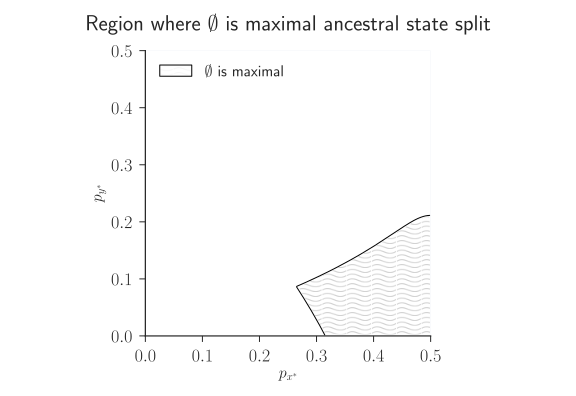
\includegraphics[width=.95\textwidth]{analytic-anc-state-inkscape}
\caption{
Region where $\emptyset$ is maximal ancestral state for each site split.
}
\label{fig:max-anc-state}
\end{figure}

The above will hold if we swap $\hat{y}_2$ and $\hat{y}_1$, as the likelihood is invariant to this.

\begin{lemma}
Let $t^*=\{x^*, y^*, x^*, y^*, y^*\}$ and $t=\{x_1, y_1, x_2, y_2, w\}$ and $\emptyset$ be the maximal ancestral state for all site splits.
The solution $\hat{t} := \{\hat{x}_1,\hat{y}_1,\hat{x}_2,\hat{y}_2,\hat{w}\}$ given by
\[
\hat{t} = \arg\max_t \ell_{\tau^*, t^*}(\tau^*, t)
\]
is subject to the constraints $\hat{x}_1,\hat{x}_2 \in [0, x^*]$, $\hat{y}_1 \in [0, y^*]$, and $\hat{y}_2,\hat{w} \in [y^*, 1]$.
\label{lemma:bounds}
\end{lemma}

\begin{proof}
We proceed by analyzing the gradients of each component of the likelihood function.
We first focus on the divergence term
\[
\shannonDivergence_{\tau^*,t^*}(\tau^*,t) = \sum_{j=1}^\nSiteSplits \Pr(\siteSplitRV=\siteSplit_j \mid \tau^*, t^*) \cdot \log \Pr(\siteSplitRV=\siteSplit_j \mid \tau^*, t).
\]
By Gibbs inequality, this function attains a unique maximum when
\[
\Pr(\siteSplitRV=\siteSplit_j \mid \tau^*, t) = \Pr(\siteSplitRV=\siteSplit_j \mid \tau^*, t^*)
\]
for all $j=1,\ldots,\nSiteSplits$ with $t^*=\{x^*,y^*,x^*,y^*,y^*\}$.
Note that exchanging $x_1$ with $x_2$ and $y_1$ with $y_2$ does not affect the divergence, and, as it has a unique maximum, we have $x_1=x_2=x$ and $y_1=y_2=y$ at this maximum.
Referring to Table~\ref{tab:sitepatprob}, we set up simultaneous equations as follows.
The sum of generating probabilities for site splits $\{3\}$ and $\{1,2\}$ yields
\[
2-2(x^*)^2 = 2-2x^2
\]
and for $\{2\}$ and $\{1,2\}$ yields
\[
2-2(y^*)^2 = 2-2y^2.
\]
implying $x=x^*$ and $y=y^*$.
Setting these parameters to their optima, the difference of generating probabilities for site splits $\emptyset$ and $\{1,3\}$ yields
\[
8x^*(y^*)^2 = 8x^*y^*w
\]
implying $w=y^*$.
The unique maximum is $\hat{t}=\{x^*,y^*,x^*,y^*,y^*\}$, and
\[
\nabla_t \shannonDivergence_{\tau^*,t^*}(\tau^*,t) \mid_{t=t^*} = 0.
\]

Assume $\emptyset$ is the most likely ancestral state for all site splits.
In this case, the partial likelihood has no ambiguity, and has terms given in Table~\ref{tab:likelihoods-restricted}.

\begin{table}
\centering
\begin{tabular}{|ll|l|}
\hline
$\siteSplit_j$ & $\ancestralSplitPartition_j(\tau, t)$ & $\Pr(\ancestralSplitRV=\xi_j \mid \siteSplitRV=\siteSplit_j,\tau,t)$\\
\hline
$\emptyset$&$\emptyset$&$(1+x_1)(1+y_1)(1+x_2)(1+y_2)(1+w)$\\
$\{1\}$    &$\emptyset$&$(1-x_1)(1+y_1)(1+x_2)(1+y_2)(1+w)$\\
$\{2\}$    &$\emptyset$&$(1+x_1)(1-y_1)(1+x_2)(1+y_2)(1+w)$\\
$\{3\}$    &$\emptyset$&$(1+x_1)(1+y_1)(1-x_2)(1+y_2)(1+w)$\\
$\{1,2,3\}$&$\emptyset$&$(1-x_1)(1-y_1)(1-x_2)(1+y_2)(1+w)$\\
$\{1,2\}$  &$\emptyset$&$(1-x_1)(1-y_1)(1+x_2)(1+y_2)(1+w)$\\
$\{1,3\}$  &$\emptyset$&$(1-x_1)(1+y_1)(1-x_2)(1+y_2)(1+w)$\\
$\{2,3\}$  &$\emptyset$&$(1+x_1)(1-y_1)(1-x_2)(1+y_2)(1+w)$\\
\hline
\end{tabular}
\caption{
The maximal likelihood values given $w=1$ and $y_2=1$.
All values multiplied by $1/32$.}
\label{tab:likelihoods-restricted}
\end{table}

We focus on $x_1$, similar arguments applying to the other variables.
The partial likelihood
\[
\tilde{\ell}_{\tau^*,t^*}(\tau^*, t) = \sum_{j=1}^\nSiteSplits \Pr(\siteSplitRV=\siteSplit_j \mid \tau^*, t^*)\cdot\log \Pr(\ancestralSplitRV=\xi_j \mid \siteSplitRV = \siteSplit_j, \tau^*, t)
\]
as a function of $x_1$, using Table~\ref{tab:sitepatprob}, is
\[
\tilde{\ell}(x_1) \propto \left(\frac{1}{2}+\frac{1}{2}x^*(y^*)^2\right)\log(1+x_1) + \left(\frac{1}{2}-\frac{1}{2}x^*(y^*)^2\right)\log(1-x_1).
\]
By some calculus, the gradient with respect to $x_1$ is
\[
\tilde{\ell}_{x_1}(x_1) = \frac{-x_1+x^*(y^*)^2}{1-x_1^2}
\]
which is clearly negative for all $x_1 \ge x^*$.
%TODO: make more explicit/clear why this means \hat{x}_1 \in [0,x^*]
This same process applied to the remaining variables shows the gradient of the full likelihood is negative for $x_1,x_2 \ge x^*$ and $y_1 \ge y^*$ and positive for $y_2,w \ge y^*$, yielding the constraints
\[
\hat{x}_1,\hat{x}_2 \in [0, x^*], \ \hat{y}_1 \in [0, y^*], \ \hat{y}_2,\hat{w} \in [y^*, 1].
\]
\end{proof}

We now prove the main result.

\topoInconsist*

\begin{proof}
%TODO: make this more explicit/clear
We use the fact that $x_1=x_2=x$ as there exists a unique solution and the likelihood is invariant to swapping these two variables.
Let
\[
a_{\emptyset} = \frac{(2x)(y_1+y_2)}{(1+x^2)(1+y_1y_2)}
\]
with similar definitions for the remaining site splits.
The objective function proportional to $w$ is
\begin{align*}
\ell(w) \propto \log(1+w) + \sum_j p_{\siteSplit_j} \log(1 + a_{\siteSplit_j}w)
\end{align*}
and has derivative with respect to $w$ as
\begin{align*}
\ell'(w) := \frac{d}{dw} \ell(w) = \frac{1}{1+w} + \sum_j p_{\siteSplit_j}a_{\siteSplit_j}\frac{1}{1 + a_{\siteSplit_j}w}.
\end{align*}
Note that, $a_{\emptyset} = -a_{13}$, $a_{2} = -a_{123}$, $p_{2} = p_{123}$, and for $x_1=x_2$
\[
a_{1} = a_{3} = a_{12} = a_{23} = 0
\]
so
\begin{align*}
\ell'(w) = \frac{1}{1+w} + \frac{p_{\emptyset}a_{\emptyset}}{1 + a_{\emptyset}w} - \frac{p_{13}a_{\emptyset}}{1 - a_{\emptyset}w} + \frac{p_{2}a_{2}}{1 + a_{2}w} - \frac{p_{2}a_{2}}{1 - a_{2}w}.
\end{align*}
Using the bounds on $\hat{x}_1,\hat{y}_1,\hat{y}_1$, and $\hat{y}_2$ from Lemma~\ref{lemma:bounds}, we have
\[
0 \le a_{\emptyset} \le \frac{2x^*}{1+(x^*)^2},
\]
\[
0 \le a_{2} \le \frac{2x^*}{1+(x^*)^2}\cdot\frac{1}{1-y^*},
\]
so that $\ell'(w)$ has lower bound
\[
\ell'_{L}(w) = \frac{1}{1+w} + - \frac{p_{13}}{c_x^* - w} - \frac{p_{2}}{c_x^*c_y^* - w}
\]
with
\[
c_x^* = \frac{1+(x^*)^2}{2x^*},
\]
\[
c_y^* = 1-y^*.
\]
The solution $\hat{w}$ solving $\ell'(w) = 0$ is greater than $\hat{w}'$ solving $\ell'_{L}(w) = 0$.
As $c_x^* > 1$, provided $c_x^*c_y^* > 1$, $\ell'_{L}(w)$ stays finite and, when considering $\ell'_{L}(w) \lessgtr 0$, we equivalently consider $f(w) \lessgtr 0$ where $f$ is the quadratic function
\begin{align*}
f(w) &= (w)^2\cdot(1+p_{13}+p_{2}) \\
      &\qquad + w\cdot(-c_x^*-c_x^*c_y^*-p_{13}c_x^*c_y^*+p_{13}-p_{2}c_x^*+p_{2}) \\
      &\qquad + ((c_x^*)^2c_y^*-p_{13}c_x^*c_y^*-p_{2}c_x^*).
\end{align*}
We see
\[
\ell'_L(0) = 1 - \frac{p_{13}}{c_x^*} - \frac{p_{2}}{c_x^*c_y^*} > 0
\]
provided again that $c_x^*c_y^* > 1$.
Now this quadratic has either zero, one, or two solutions.
If there are zero solutions, the derivative with respect to $w$ is increasing on all of $[0,1]$ so that $\hat{w} = 1$ and we are done.
If there are one or two solutions,
if the smaller of the zeros of $f(w)$ is greater than one, then $\hat{w} \equiv 1$.
Using the quadratic formula with
\[
a = 1+p_{13}+p_{2},
\]
\[
b = -c_x^*-c_x^*c_y^*-p_{13}c_x^*c_y^*+p_{13}-p_{2}c_x^*+p_{2},
\]
\[
c = (c_x^*)^2c_y^*-p_{13}c_x^*c_y^*-p_{2}c_x^*,
\]
the smaller zero is
\[
\hat{w} = \frac{-b - \sqrt{b^2 - 4ac}}{2a},
\]
which is a function of the generating parameters $x^*$ and $y^*$.
We see that $a \ge 0$ and, provided that $2a+b \leq 0$, we have,
\[
\hat{w} \ge 1 \iff
|2a + b| \leq \sqrt{b^2 - 4ac} \iff
%-b - \sqrt{b^2 - 4ac} \le 2a,
%0 \ge -b - 2a \le \sqrt{b^2 - 4ac},
%b^2 + 4ab + 4a^2 \le b^2 - 4ac,
%a^2 + ab + ac \le 0,
a + b + c \ge 0.
\]
Therefore, we have three conditions to satisfy for $\hat{w} \equiv 1$:
\[
\mathrm{C}1: c_x^*c_y^* > 1,
\]
\[
\mathrm{C}2: 2-c_x^*c_y^*-c_x^*+p_{13}(3-c_x^*c_y^*)+p_{2}(3-c_x^*) \leq 0,
\]
\[
\mathrm{C}3: 1+(c_x^*)^2c_y^*-c_x^*c_y^*-c_x^*+p_{13}(2-2c_x^*c_y^*)+p_{2}(2-2c_x^*) \ge 0.
\]
The set of $x^*,y^*$ satisfying these conditions as well as those for $\emptyset$ being the most likely ancestral state is given in Figure~\ref{fig:incons-analytic}.
\end{proof}

As the region in Figure~\ref{fig:incons-analytic} gives the values of $x^*$ and $y^*$ where $\hat{w}$ is guaranteed to be one, we converge on the incorrect topology in these cases, resulting in an inconsistency.

\subsection*{Empirical validation}

Consider Table~\ref{tab:likelihoods}.
There are 81 separate possible forms for the likelihood, corresponding to the three possible most likely ancestral states for each of the four ambiguous site splits.
In Fig.~\ref{fig:bl-general-inconsistency}, for various values of $x^*,y^*$, we compute the maximum of each of the 81 likelihoods and plot the value of $\hat{p}_w = (1-\hat{w})/2$.

\begin{figure}
\centering
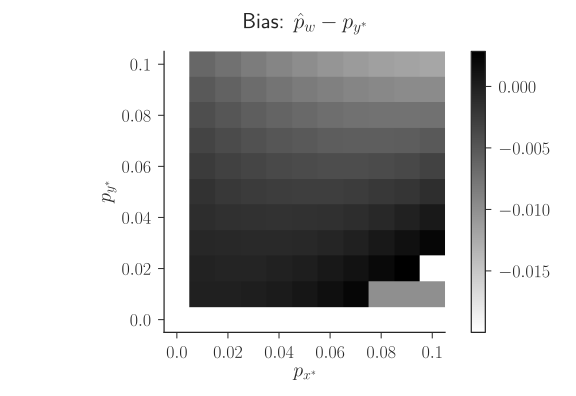
\includegraphics[width=.95\textwidth]{empirical-bias}
\caption{
Bias in branch length estimation.
In regions where joint optimization should perform well, there is systematic bias toward shorter branch lengths.
}
\label{fig:empirical-bias}
\end{figure}


\begin{figure}
\centering
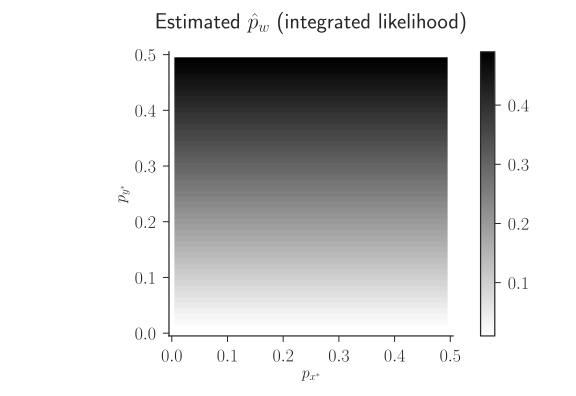
\includegraphics[width=\textwidth]{empirical-marginal}
\caption{
    Estimates for $\hat{p}_w$ when computing $(\hat{x}, \hat{y}, \hat{w})$ using L-BFGS-B optimizing the classical marginal likelihood \eqref{eq:marginal_likelihood} (rather than a joint optimization procedure).
}
\label{fig:bl-general-marginal}
\end{figure}
%
%\begin{figure}
%\centering
%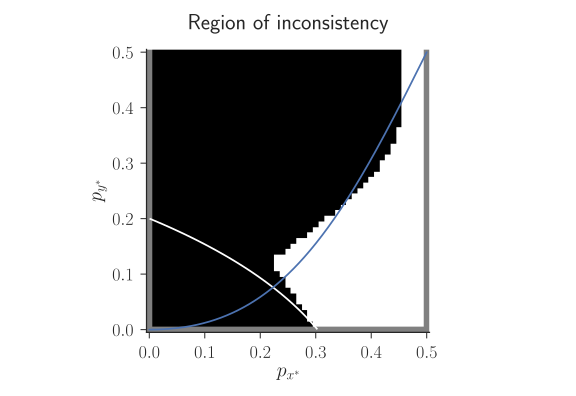
\includegraphics[width=.95\textwidth]{empirical-incons-intuition}
%\caption{
%Inconsistency in joint inference with intuitive curves.
%The white curve is our condition on the gradients.
%The blue curve is a condition on $x^*$ and $y^*$ such that $\emptyset$ is the most likely ancestral state.
%}
%\label{fig:empirical-incons-intuition}
%\end{figure}

